\documentclass{article}

% Document extensibility %
%
% Disables native paragraph indentation
\usepackage{parskip} 
%
% Provides further bullet options for lists
\usepackage{enumitem}

% Mathematical symbol and statement packages %
%
% Necessary
\usepackage{amsmath}
\usepackage{amssymb}
%
% Extensive fraction notation
\usepackage{xfrac}
%
% Generic mathematical commands
% Notable: \degree, \celcius
\usepackage{gensymb}
%
% Variable vector notation (arrow above variable)
\usepackage{esvect}
%
% Multiline boxed equations
\usepackage{empheq}
%
% SI Unit
\usepackage{siunitx}
%
% More intuitive arrays/matrices
\usepackage{array}

% Graphic packages %
%
% Diagrams and illustrations
\usepackage{tikz}
%
% Image insertion
\usepackage{graphicx}
\graphicspath{ {./} }

% Document content %
%
% Change title of table of contents
% \renewcommand{\contentsname}{Title}

\begin{document}

% Command `\hr` to insert horizontal rules
\newcommand{\hr}{\par\noindent\rule{\textwidth}{0.4pt}}

% Command to box and center math equations
\newcommand{\bc}[1]{
	\begin{equation*}
		\begin{boxed}
			{#1}
		\end{boxed}
	\end{equation*}
}

% Command for single line equations with a condition
\newcommand{\cond}[2]{
	\ifmmode
		{#1} \quad {#2}
	\else
		$$ {#1} \quad {#2} $$
	\fi
}

\section{Friction}

\subsection{Example 1}

\subsection{Example 2}
\begin{align*}
	\mu_R & = 0.1 \\
	\mu_{\text{max}} & = 0.3 \\
	m & = \SI{1}{\kilogram} \\
	\theta & = \SI{15}{\degree}
\end{align*}
What is the range of force values for which the system is static?
\begin{align*}
	\sum F_x^{\text{min}} & = 0 \\
	N & = F_{\text{min}}\sin(\theta)
\end{align*}
\begin{align*}
	\sum F_y^{\text{min}} & = 0 \\
	f_{\text{min}} + F_{\text{min}}\cos(\theta) & = mg \\
	\mu_{\text{max}}(F_{\text{min}}\sin(\theta)) + F_{\text{min}}\cos(\theta) & = mg \\
	F_{\text{min}} & = \frac{mg}{\cos(\theta) + \mu_{\text{max}}\sin(\theta)} \\
	\therefore \quad F_{\text{max}} & = \frac{mg}{\cos(\theta) - \mu_{\text{min}}\sin(\theta)}
\end{align*}

\subsection{Example 3}
\begin{align*}
	F & = ? \\
	m_1 & = \SI{10}{\kilogram} \\
	\mu_k & = 0.1 \\
	m_2 & = \SI{5}{\kilogram} \\
	\mu_{\text{max}} & = 0.4 \\
	a & = ?
\end{align*}

\subsection{Example 4}
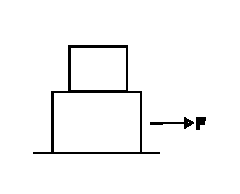
\includegraphics{"./drawing.eps"}
\begin{align*}
	m_1 & = \SI{2}{\kilogram} \\
	m_2 & = \SI{5}{\kilogram} \\
	u_{\text{max}} & = 0.5 \\
	u_k & = 0.2 \\
	a_\text{bottom}  & = a_\text{top} = a \\
	F & = ?
\end{align*}
How much force is needed to move the bottom block while the top stays static?
\begin{align*}
	\sum F_y^{(m_2 + m_1)} & = 0 \\
	N_{g,b} & = (m_1 + m_2)g
\end{align*}
\begin{align*}
	\sum F_x^{(m_2 + m_1)} & = 0 \\
	F & = f_{g,b} \\
	F & = \mu_\text{max}N_{g,b} \\
	F & = \mu_\text{max}(m_2 + m_1)g \\
	F & = 0.5(\SI{70}{\newton}) \\
	F & = \SI{35}{\newton}
\end{align*}
\begin{align*}
	\sum F_y^{(m)} & = 0 \\
	N_{t,b} & = mg
\end{align*}
\begin{align*}
	\sum F_x^{(m)} & = ma \\
	f_{t,b} & = ma \\
	a & = \frac{f_{t,b}}{m} \\
	a & = \frac{\mu_\text{max}mg}{g} \\
	a & = \mu_\text{max}g = (0.5)(\SI{10}{\meter \per \second \squared}) \\
	a & = \SI{5}{\meter \per \second \squared}
\end{align*}
\begin{align*}
	\sum F_y^{(m_2 + m_1)} & = 0 \\
	N_{g,b} & = (m_1 + m_2)g = \SI{70}{\newton}
\end{align*}
\begin{align*}
	\sum F_x^{(m_2 + m_1)} & = (m_2 + m_1)a \\
	F - f_{g,b} & = (m_2 + m_1)a \\
	F & = (m_1 + m_2)a + \mu_kN_{g,b} \\
	F & = \SI{49}{\newton}
\end{align*}

\end{document}
